\section{Simulation Studies}\label{sec:simulation}
We assess the finite sample properties of our proposed spectral density estimators through numerical experiments on simulated data sets. To this end, we compare the performance of smoothed periodogram, shrinkage estimator from \cite{bohm2009shrinkage},  hard thresholding, soft thresholding (lasso) and adaptive lasso thresholding. In particular, we simulate data from vector moving average (VMA) and autoregressive (VAR) processes with block-diagonal transition matrices and evaluate estimation and model selection performance of these methods for different values of $n$ and $p$. Overall, the results demonstrate that thresholding methods provide substantial improvements in estimation accuracy over smoothed periodograms and shrinkage methods when $p$ is large and the true spectral density is approximately sparse. In addition, thresholding methods accurately recovers the edges in coherence networks, as measured by their precision, recall and area under receiver operating characteristic (ROC)  curves. 

\textit{Generative models: } { We consider VAR(1) models $X_t = A X_{t-1} + \varepsilon_t$  of three different dimensions: $p =12, 48, 96$. Each element in $\varepsilon_t$ is independent and identically distributed as $\mathcal{N}(0,1)$, and the transition matrix $A$ is composed of $3 \times 3$ block matrices on the diagonal. Each block matrix $A^0$ has $0.5$ on the diagonal and $0.9$ on the first upper off-diagonal. We also consider VMA(1) models $X_t = B \varepsilon_{t-1}+\varepsilon_t$ of the same dimensions as the VAR models. These transition matrix structures are adopted from \citet{fiecas2014datadriven}, where a data-driven shrinkage method was shown to improve upon smoothed periodograms in high-dimensional settings. For each model, we generate $n =100, 200, 400, 600$ consecutive observations from the multivariate time series.}

%We evaluate the performance for different methods for both VAR and VMA models. We focus on transition matrices in both model as the block diagonal matrices. We test two settings: one is with homogeneous blocks and the other have heterogeneous blocks. In this setting, each transition/weight matrix shares the same block size and value. 

The transition matrix $A$ of VAR is a block diagonal composed of identical blocks consisting of a $3 \times 3$ upper triangular matrix $A^0$. 
Similarly, the VMA transition matrix $B$ is a block diagonal matrix composed of identical $3 \times 3$ upper triangular matrix $B^0$.

\begin{equation}
A^0 = B^0 = \left[ \begin{array}{ccc} 
0.5 & 0.9 & 0  \\ 
0 & 0.5 & 0.9  \\
0 & 0 & 0.5  \\
\end{array}\right].
\end{equation} 


%\paragraph In the {\textit{heterogeneous setting}, }
%$A_1$ is initialed the same as the one in homogeneous setting. To add heterogeneity to it, the first block is replaced by a independent structure with 0.1 on the diagonal. 
%the VAR transition matrix $A$ is also block diagonal, but consists of two blocks with unequal sizes $2p/3$ and $p/3$. The larger block is upper triangular with each entry  equal to $0.1$, and the smaller block is symmetric with 0.1 on the diagonal and -0.3 elsewhere. The VMA transition matrix $B$ is a block diagonal matrix composed of two block matrices with size $2p/3$ and $p/3$, where $B_1^1$ has an independent structure with 0.4 on the diagonal, $B_1^2$ an exchangeable structure with 0.4 on the diagonal and -0.5 off the diagonal. More details about the transition matrices can be found in Appendix  \ref{sec:simulation_setting}. {\color{red} [Yiming: why did VAR and VMA network topologies differ in heterogeneous setting?] } 


% \subsection{Evaluation}

%\subsubsection{Ground truth}
The estimated spectral density matrices are compared to the true spectral densities. For stable, invertible VARMA(1,1) processes $X_t = AX_{t-1} + 
  %A_2X_{t-2} + \cdots + A_d X_{t-d} +
  \varepsilon_t 
  + B\varepsilon_{t-1}
  %- B_2\varepsilon_{t-2} - \cdots - B_{\ell}\varepsilon_{t-\ell}.
$, true spectral densities take the form 
\begin{equation*}
f(\omega) = \frac{1}{2\pi} (\mathcal{A}^{-1}(e^{-i\omega}))\mathcal{B}(e^{-i\omega})\Sigma_{\varepsilon}\mathcal{B}^{\dag}(e^{-i\omega})(\mathcal{A}^{-1}(e^{-i\omega}))^{\dag},
\end{equation*}

where $\mathcal{A}(z) = I_p - A z$ and $\mathcal{B}(z) = I_p +  B z$.

\smallskip
\textit{Performance Metrics: } We compare the estimation performances of different estimators of  $f(\omega_j)$ using Relative Mean Integrated Squared Error (RMISE) in Frobenius norm, defined as
 \begin{equation*}
{RMISE}(\hat{f}) := \frac{\sum_{j\in F_n} \|\hat{f}(\omega_j) - f(\omega_j)\|_F^2}{\sum_{j\in F_n} \|f(\omega_j)\|_F^2}. 
\end{equation*}
% We choose the relative error instead of MISE to better compare the accuracy of the estimates relative to a null model across different values of $p$. 

In order to capture how well the three thresholding methods recover the non-zero coordinates in a spectral density matrix under exactly sparse generative VMA and VAR models, we also record their precision, recall and F1 measures over all Fourier frequencies %In particular, we used 
\begin{eqnarray}
    && \text{precision}(\omega_j) = % n^{-1}\sum_{j  \in F_n} 
    \frac{\# \{(r,s): ~ |\hat{f}_{rs}(\omega_j)|\neq 0, ~ |f_{rs}(\omega_j)|\neq 0 \}}{\# \{(r,s): ~ |\hat{f}_{rs}(\omega_j)|\neq 0\}} \nonumber \\
    && \text{recall}(\omega_j) = \frac{\# \{(r,s): ~ |\hat{f}_{rs}(\omega_j)|\neq 0, ~ |f_{rs}(\omega_j)|\neq 0 \}}{\# \{(r,s): ~ |f_{rs}(\omega_j)|\neq 0\}} \nonumber \\
    && \text{F1}(\omega_j) =  2\times (\text{precision}(\omega_j) \cdot \text{recall}(\omega_j))/(\text{precision}(\omega_j) + \text{recall}(\omega_j)). \nonumber 
\end{eqnarray}
We calculate each of the three criteria averaged across all Fourier frequencies $j\in F_n$.  All the experiments are replicated  $50$ times, and mean and standard deviation of the performance metrics are reported. 


We also evaluate the accuracy of thresholding methods in selecting the graph $G = \{ (r,s) \in V \times V: \hat{f}_{rs}(\omega_j) \neq 0 \mbox{ for some } \omega_j \in F_n \}$. For this purpose, we use averaged absolute coherence (across all Fourier frequencies) to construct a single $p \times p$ weighted adjacency matrix $\hat{G}$, and then measure its accuracy in selecting edges of the true graph $G$. \par 

\textit{Tuning parameter selection: } For each of the three thresholding methods, we use the sample-splitting algorithm \ref{alg:sample-split} with $N = 1$ to determine the value of threshold for individual frequencies. We choose a  grid $\mathcal{L}$ of equispaced values between the minimum and maximum moduli of off-diagonal entries in smoothed periodogram.  Based on the theoretical considerations in Section \ref{sec:theory}, the smoothing spans for VMA models are chosen by setting $m = \sqrt{n}$. Since $\Omega_n(f)$ is  larger for VAR than VMA models considered here, a smaller  smoothing span is chosen by setting $m = 2/3\sqrt{n}$. The results are qualitatively similar in our sensitivity analysis with different values of $m$ of this order. 

\textit{Results: } The RMISE of smoothed (averaged) periodograms, shrinkage and thrsholding methods are reported in Table \ref{table:rmise-homogeneous-final}. The results show that both shrinkage and thresholding outperform smoothed periodogram, and the improvement is more prominent for larger $p$. Further, thresholding procedures show some improvement over shrinkage methods in these approximately sparse data generative models. Amongst the three thresholding methods,  lasso and adaptive lasso tend to have lower error than hard thresholding in most settings. 

Precision, recall and F1 scores of the three thresholding methods are reported 
%in Table \ref{table:precision-homogeneous-final} 
in Appendix \ref{appendix:more_tables}. In most of the simulation settings, the methods have high precision but low recall, indicating higher true negative in general. This matches with our theoretical predictions for weakly sparse spectral densities in Proposition \ref{prop:consistency}. The F1 scores are in the range of $50-60\%$ in most simulation settings. As in the RMISE results, lasso and adaptive lasso thresholds perform significantly better than hard thresholding in most simulation settings.



The ROC curves for the three thresholding methods in selecting coherence graph of a VAR(1) model with $p=48$ and $n \in \{100, 200, 400, 600\}$ are provided in Figure \ref{fig:roc}. Consistent with the frequency-specific precision and recall results, lasso and adaptive lasso thresholding methods perform better than hard thresholding. 

Overall, our numerical experiments confirm that thresholding procedures can be successfully used to estimate large spectral density matrices with same order of accuracy as shrinkage methods, and with an additional advantage of performing automatic edge selection in coherence networks.  


\begin{table}
%\def~{\hphantom{0}}
\begin{tabular}{l@{\hskip 0.4in}ccccc}
%\\
\\
& Smoothed   & Shrinkage & Hard Threshold  & Lasso & Adaptive Lasso\\
\\
VMA & & & & &\\
p = 12 & & & & &\\
\multicolumn{1}{r}{n = 100}&43.21(6.86)&22.15(1.77)&27.43(2.11)&22.89(2.05)&25.54(1.91)\\
\multicolumn{1}{r}{n = 200}&29.95(2.93)&17.67(1.01)&20.5(1.45)&16.18(1.33)&18.74(1.32)\\
\multicolumn{1}{r}{n = 400}&21.11(1.75)&14.24(0.67)&12.39(1.52)&10.84(1.01)&11.33(1.27)\\
\multicolumn{1}{r}{n = 600}&17.28(1.39)&12.58(0.59)&8.73(1.16)&8.84(0.71)&8.45(0.92)\\
p = 24 & & & & &\\
\multicolumn{1}{r}{n = 100}&80.49(7.63)&26.28(1.62)&29.86(1.21)&26.36(1.5)&28.38(1.31)\\
\multicolumn{1}{r}{n = 200}&59.79(4.7)&22.92(0.81)&25.62(0.86)&19.29(1.35)&22.09(1.21)\\
\multicolumn{1}{r}{n = 400}&41.83(1.98)&19.54(0.45)&17.16(1.26)&13.0(0.99)&13.71(1.25)\\
\multicolumn{1}{r}{n = 600}&35.86(1.6)&17.83(0.36)&12.27(1.01)&10.36(0.65)&9.89(0.84)\\
p = 48 & & & & &\\
\multicolumn{1}{r}{n = 100}&162.79(9.94)&29.58(1.24)&30.62(0.91)&28.78(0.83)&29.9(0.8)\\
\multicolumn{1}{r}{n = 200}&119.58(4.21)&27.0(0.57)&28.29(0.37)&22.68(0.76)&25.48(0.72)\\
\multicolumn{1}{r}{n = 400}&83.48(2.67)&24.09(0.37)&22.35(0.65)&15.86(0.54)&17.21(0.74)\\
\multicolumn{1}{r}{n = 600}&69.83(1.77)&22.58(0.28)&16.95(0.81)&12.88(0.48)&12.73(0.7)\\
p = 96 & & & & &\\
\multicolumn{1}{r}{n = 100}&324.57(14.7)&32.34(1.15)&30.3(0.46)&29.71(0.43)&30.11(0.44)\\
\multicolumn{1}{r}{n = 200}&235.78(7.75)&29.58(0.67)&28.83(0.28)&25.28(0.43)&27.31(0.38)\\
\multicolumn{1}{r}{n = 400}&167.89(4.28)&27.44(0.37)&25.67(0.33)&18.58(0.5)&20.34(0.55)\\
\multicolumn{1}{r}{n = 600}&139.4(2.02)&26.26(0.24)&21.25(0.48)&15.35(0.37)&15.72(0.51)\\
VAR & & & & &\\
p = 12 & & & & &\\
\multicolumn{1}{r}{n = 100}&39.11(10.1)&37.49(5.27)&41.09(6.36)&38.46(5.25)&41.81(5.18)\\
\multicolumn{1}{r}{n = 200}&28.06(8.4)&25.2(4.15)&30.52(5.83)&27.6(4.19)&30.69(5.21)\\
\multicolumn{1}{r}{n = 400}&17.31(4.63)&16.51(2.93)&19.37(3.74)&16.84(2.61)&19.5(3.41)\\
\multicolumn{1}{r}{n = 600}&25.0(5.86)&19.23(3.95)&23.07(4.62)&18.55(2.85)&21.65(3.92)\\
p = 24 & & & & &\\
\multicolumn{1}{r}{n = 100}&73.83(15.52)&49.25(4.16)&49.18(4.78)&44.64(3.8)&47.59(3.54)\\
\multicolumn{1}{r}{n = 200}&54.77(9.83)&36.84(2.97)&40.95(3.46)&34.29(3.52)&38.46(3.47)\\
\multicolumn{1}{r}{n = 400}&35.53(6.01)&27.34(2.05)&27.43(2.86)&22.32(1.76)&25.05(2.67)\\
\multicolumn{1}{r}{n = 600}&28.53(2.24)&21.82(0.74)&17.25(0.97)&15.17(0.11)&16.64(0.98)\\
p = 48 & & & & &\\
\multicolumn{1}{r}{n = 100}&131.88(20.49)&61.75(4.11)&49.3(3.35)&47.12(1.89)&48.1(2.25)\\
\multicolumn{1}{r}{n = 200}&99.46(12.68)&48.3(2.17)&44.24(1.53)&39.31(1.77)&42.63(1.41)\\
\multicolumn{1}{r}{n = 400}&69.19(7.07)&38.38(1.44)&35.52(1.55)&26.69(1.35)&30.5(1.75)\\
\multicolumn{1}{r}{n = 600}&53.08(1.38)&32.58(0.4)&25.23(0.41)&20.38(0.3)&21.16(0.52)\\
p = 96 & & & & &\\
\multicolumn{1}{r}{n = 100}&259.85(31.63)&75.46(5.47)&48.6(1.69)&47.96(1.41)&48.15(1.59)\\
\multicolumn{1}{r}{n = 200}&200.12(16.87)&59.45(1.88)&45.18(1.23)&43.34(1.2)&44.63(1.06)\\
\multicolumn{1}{r}{n = 400}&135.52(8.76)&50.08(1.25)&41.41(0.7)&32.53(1.11)&37.13(1.14)\\
\multicolumn{1}{r}{n = 600}&97.13(1.32)&42.62(0.08)&31.65(0.45)&24.6(0.34)&24.56(0.69)\\
\end{tabular}
\label{table:rmise-homogeneous-final}
\caption{Relative Mean Integrated Squared Error (RMISE, in \%) of smoothed periodogram, shrinkage towards a diagonal target and three different thresholding methods - hard thresholding, lasso and adaptive lasso. Results are averaged over $20$ replicates. Standard deviations (also in \%) are reported in parentheses.}
\end{table}


\begin{figure}[!t]
    \centering
    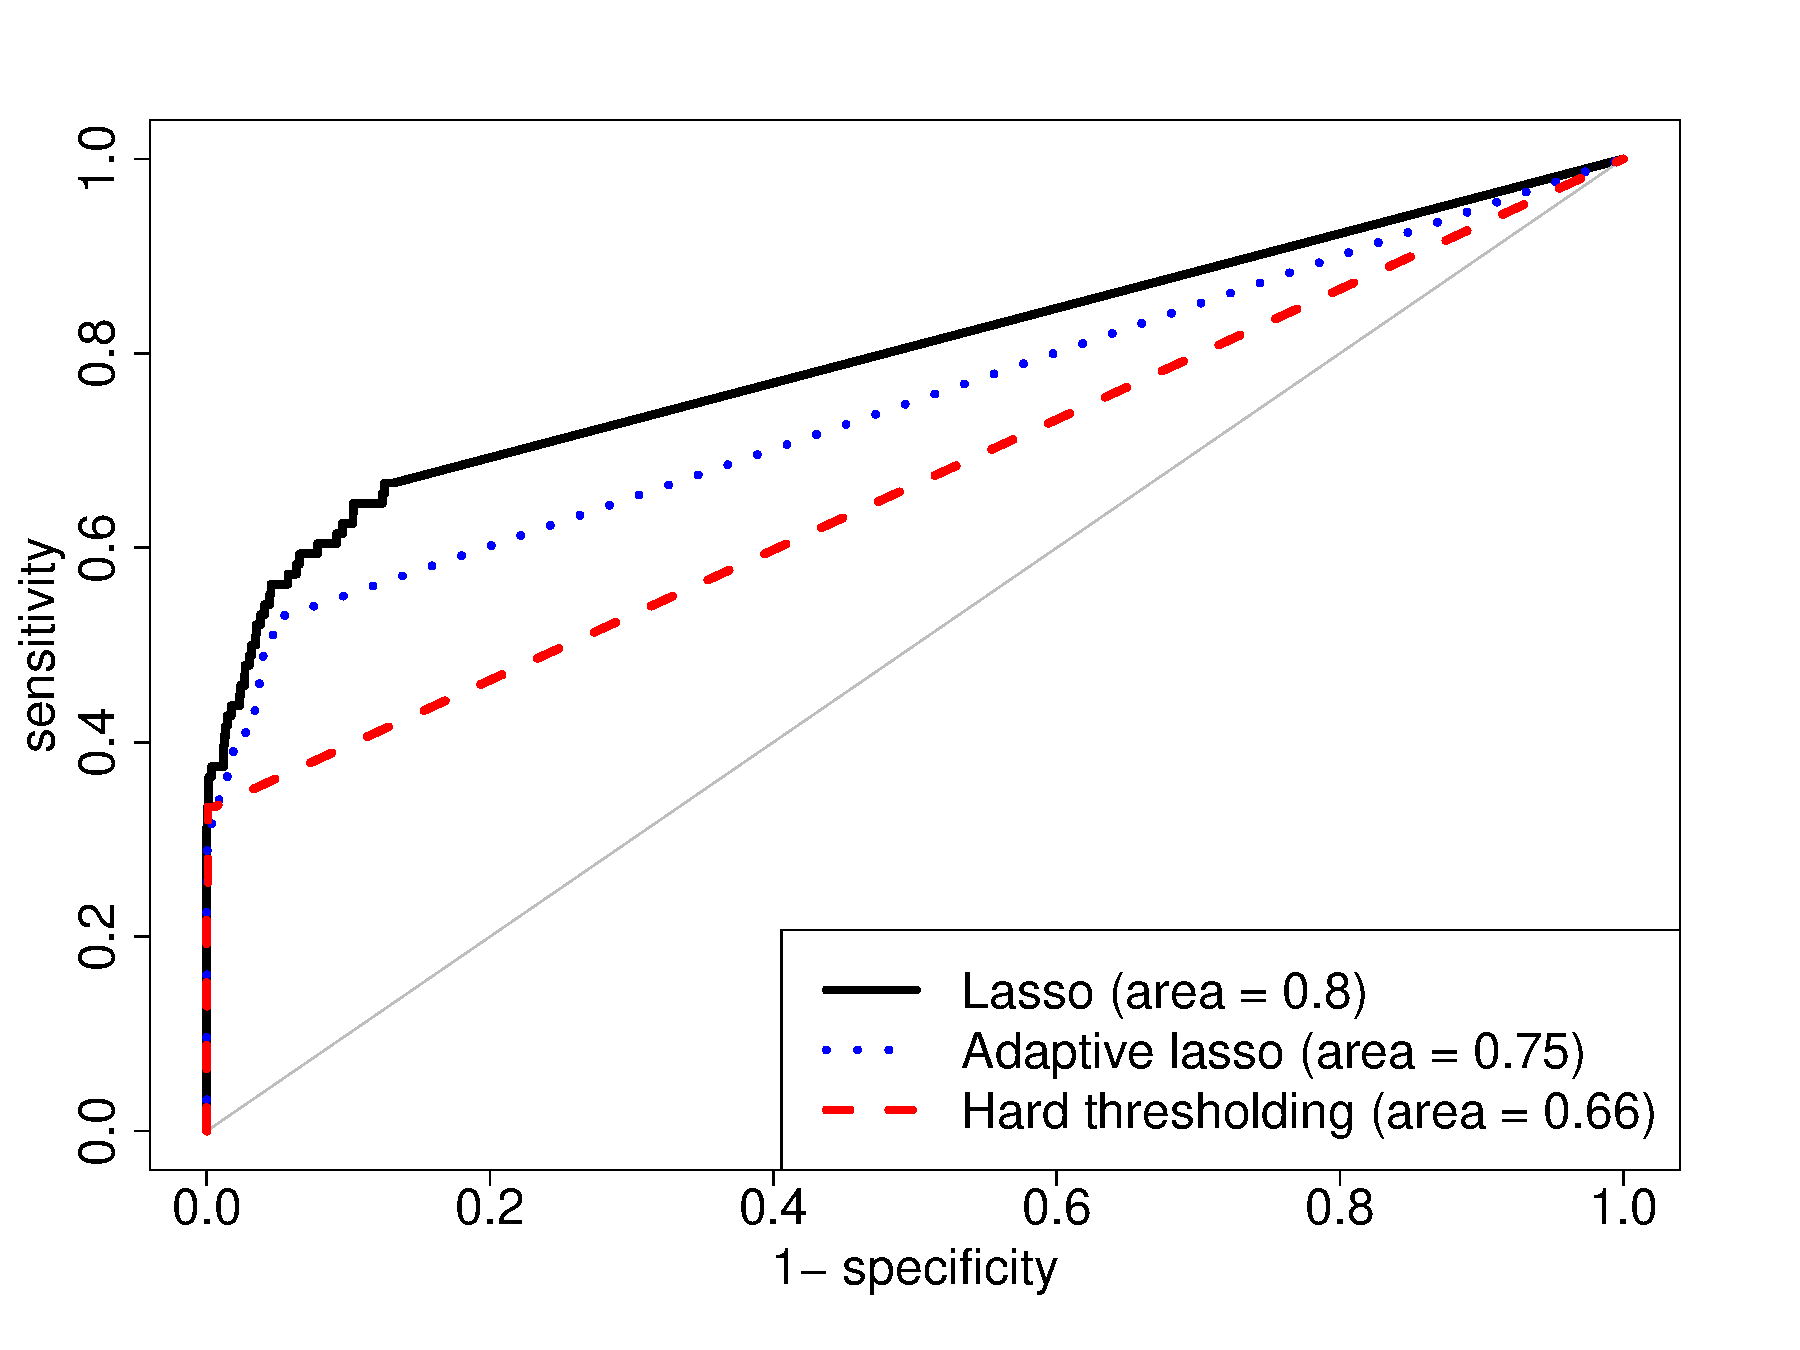
\includegraphics[width=0.48\textwidth]{img/ROC_100_96.pdf}
    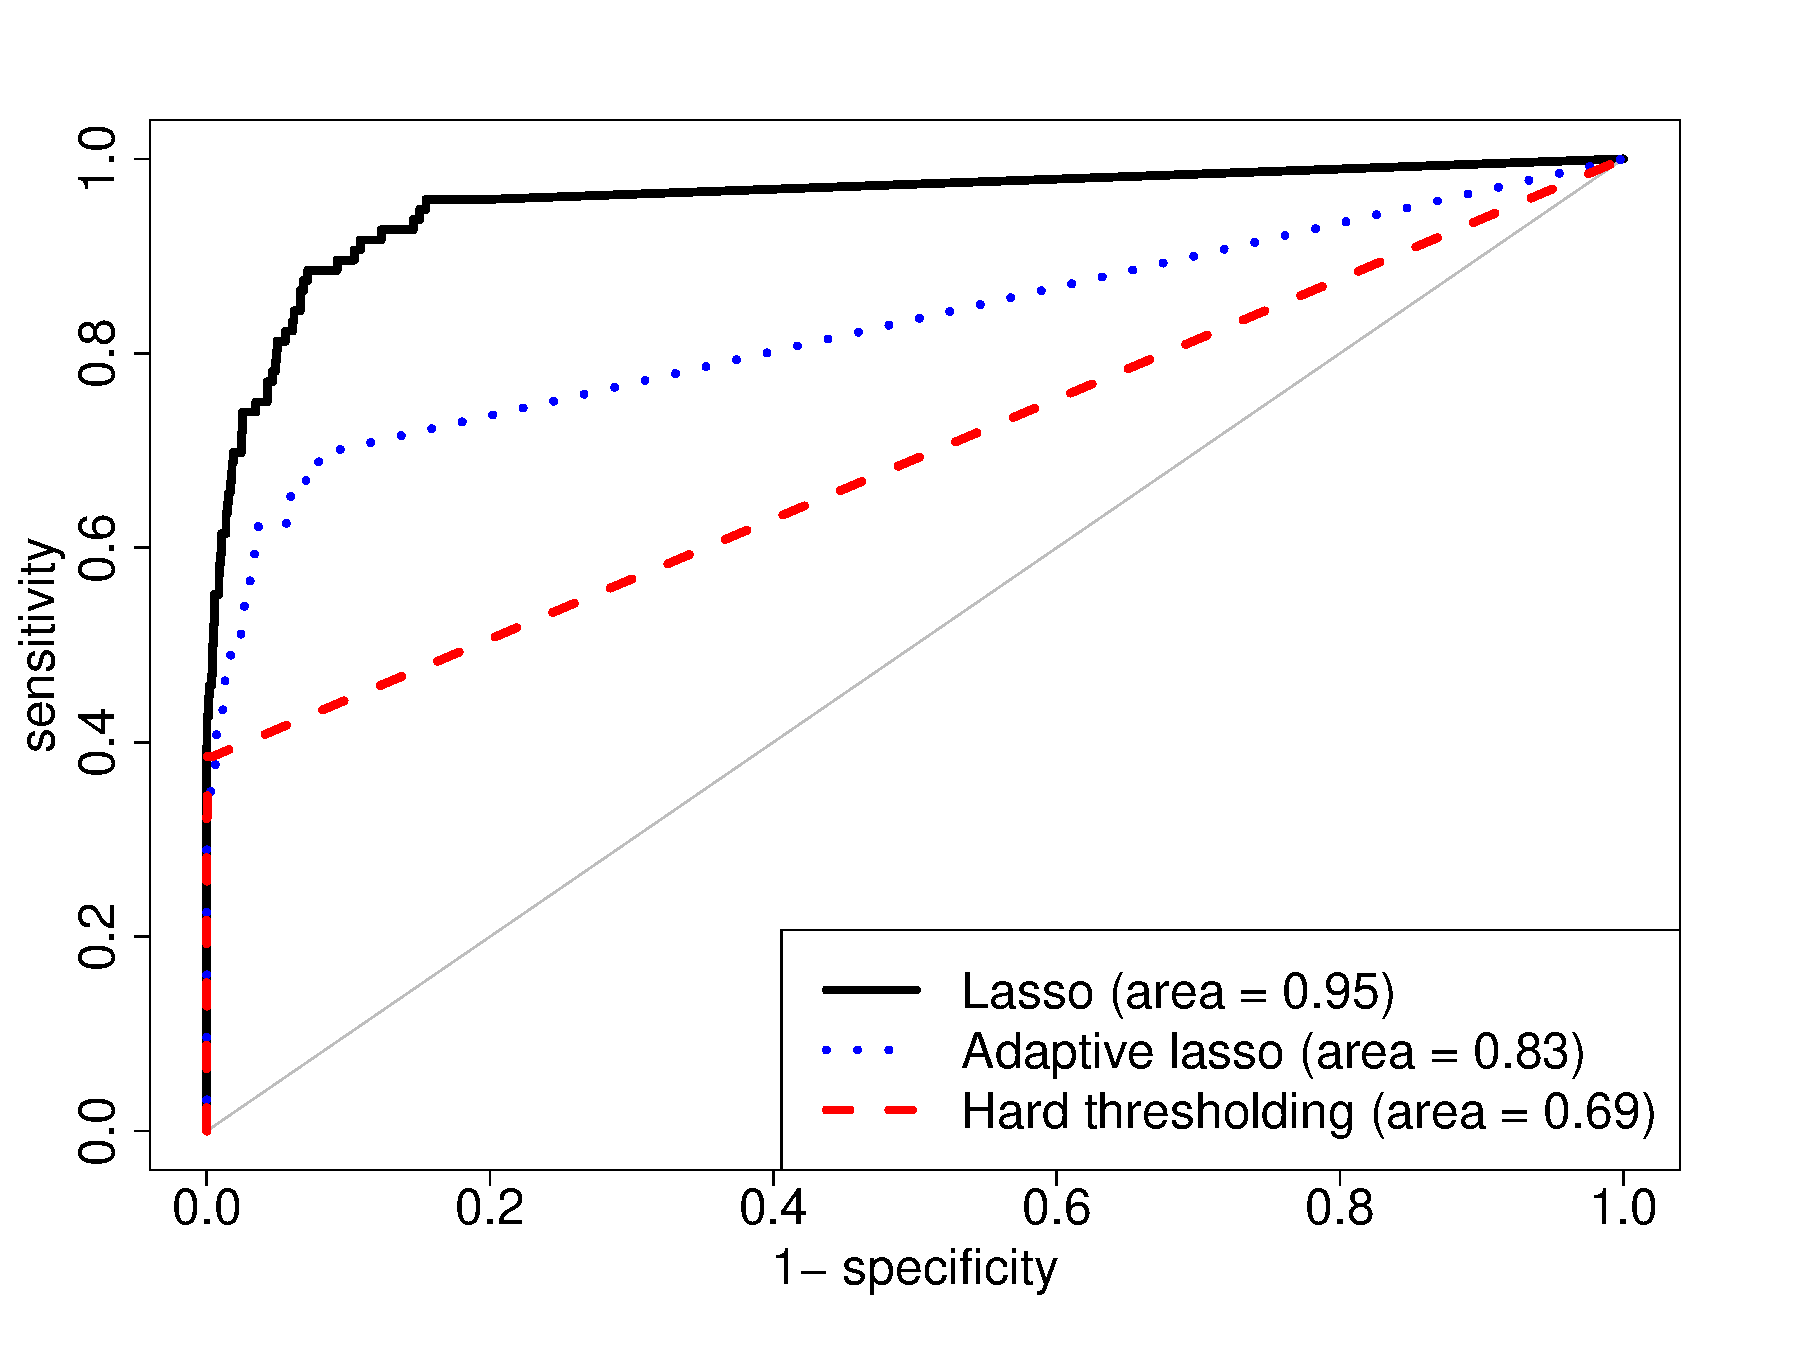
\includegraphics[width=0.48\textwidth]{img/ROC_200_96.pdf}
    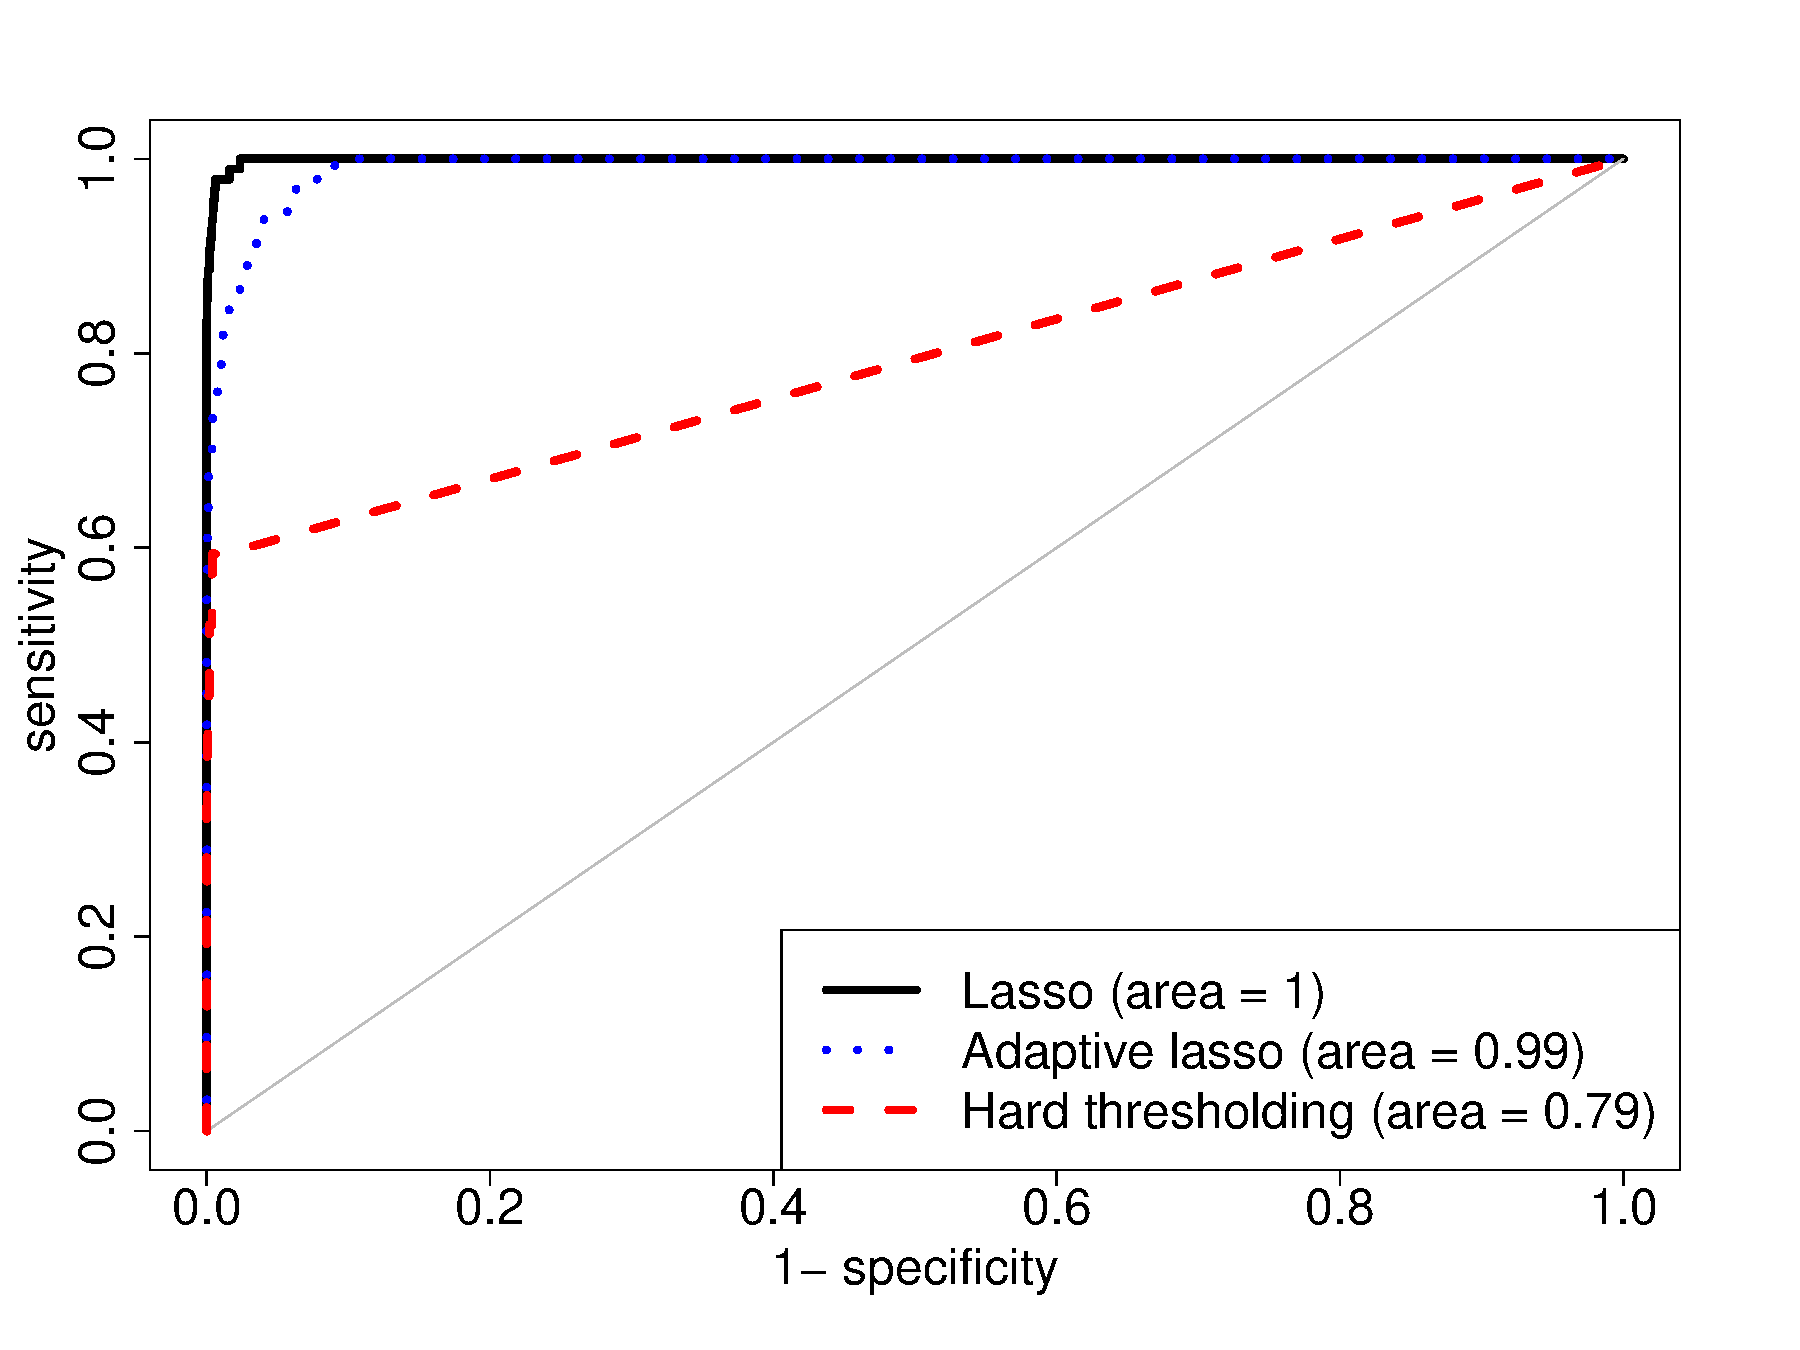
\includegraphics[width=0.48\textwidth]{img/ROC_400_96.pdf} 
    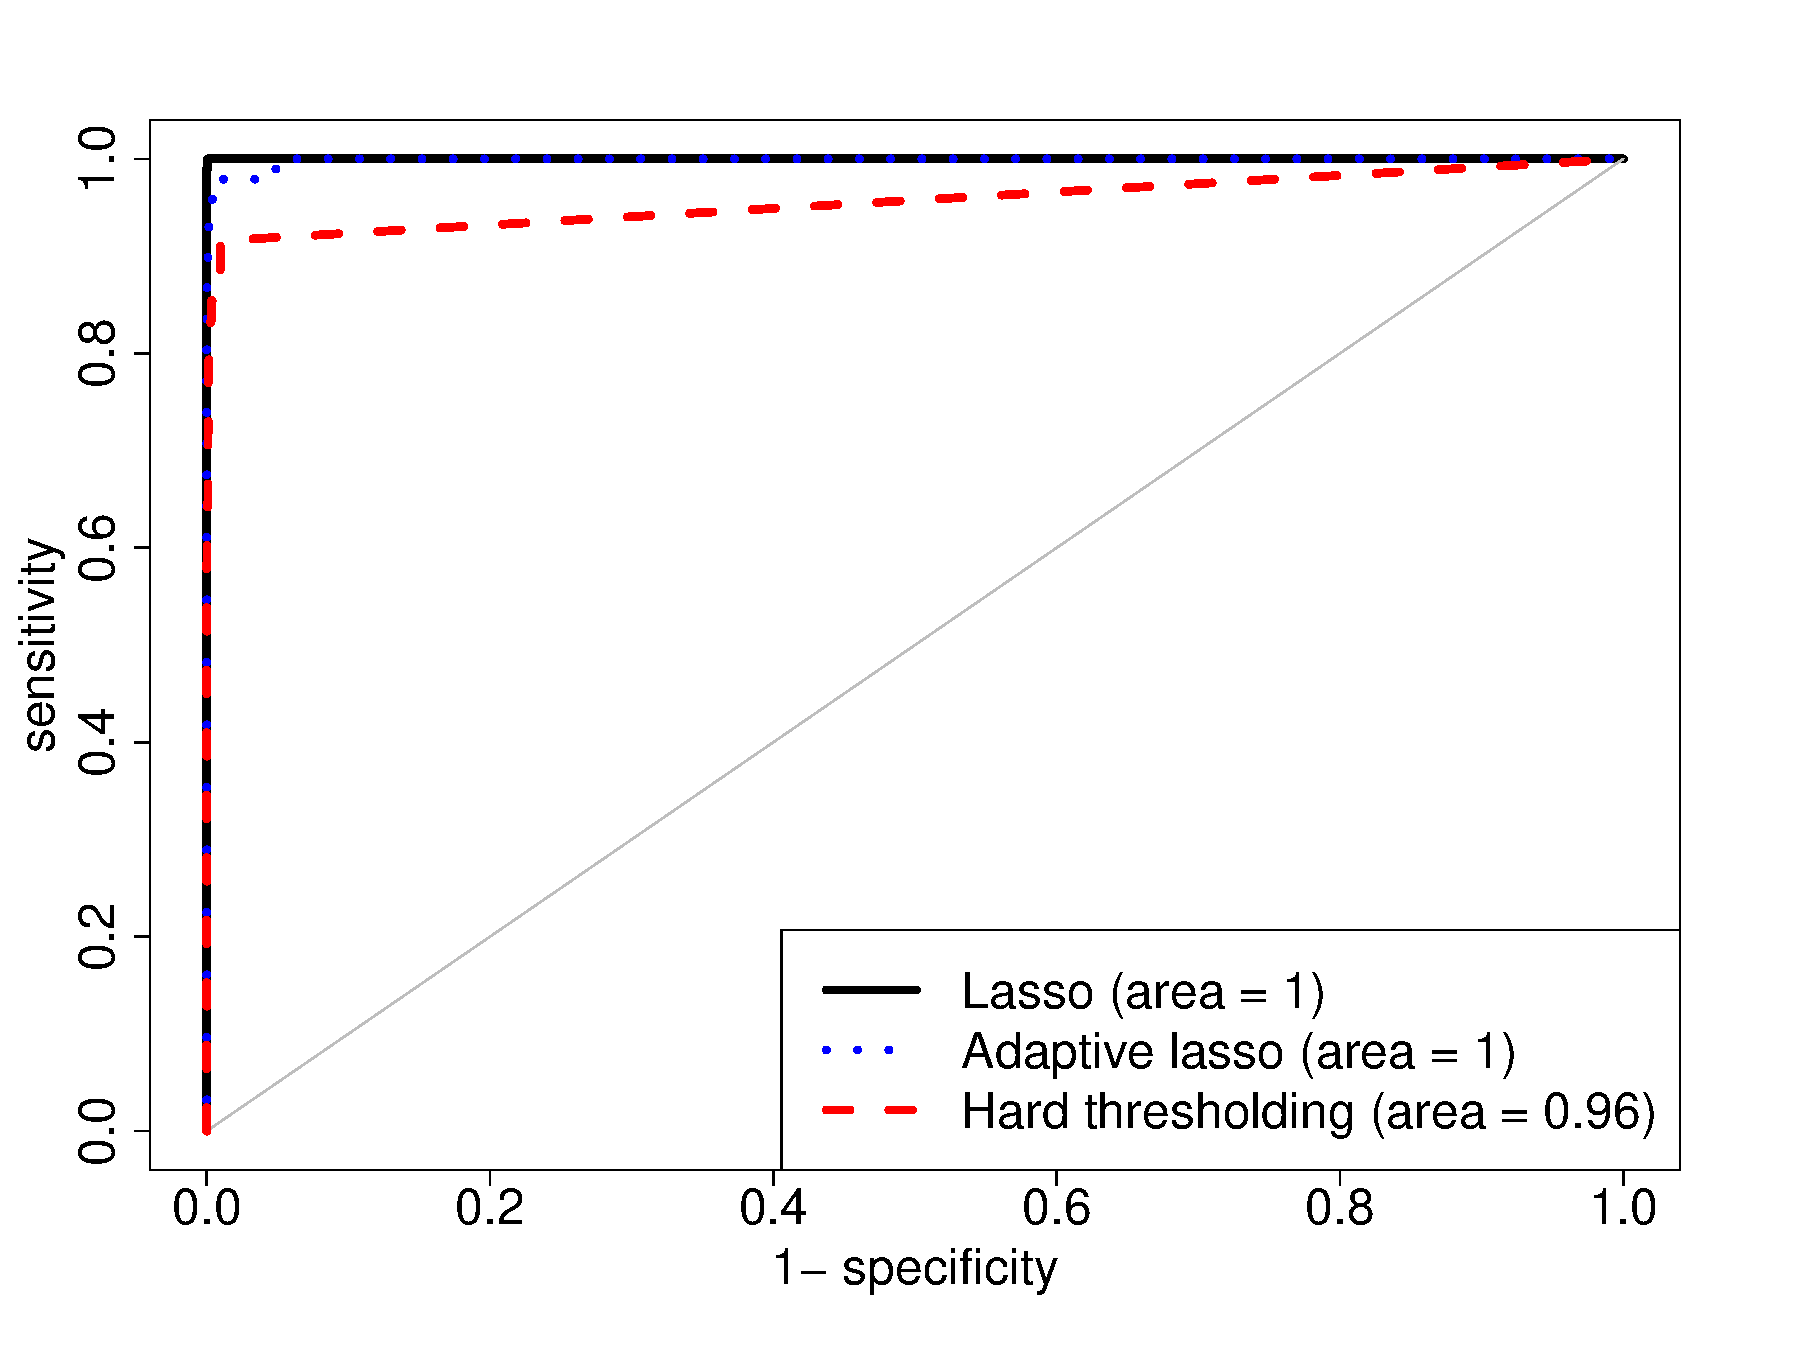
\includegraphics[width=0.48\textwidth]{img/ROC_600_96.pdf}    
    \caption{Receiver Operating Characeristic (ROC) curves of hard thresholding, lasso and adaptive lasso for recovering coherence network of a $p = 96$ dimensional VAR(1) model using $n = 100$ (top left), $n = 200$ (top right), $n = 400$ (bottom left) and $n = 600$ (bottom right) time series observations.}
    \label{fig:roc}
\end{figure}


% The results for heterogeneous settings are reported in Tables \ref{table:rmise-heterogeneous} and \ref{table:precision-heterogeneous}. Compared to homogeneous setting, RMISE of the three thresholding based methods outperform shrinkage estimators by a larger margin. {\color{red} [Sumanta: add description of precision/recall, and Figure \ref{fig::hetero}]. }




%\subsection{Tables and Graphs}



